%Version 3.1 December 2024
% See section 11 of the User Manual for version history
%
%%%%%%%%%%%%%%%%%%%%%%%%%%%%%%%%%%%%%%%%%%%%%%%%%%%%%%%%%%%%%%%%%%%%%%
%%                                                                 %%
%% Please do not use \input{...} to include other tex files.       %%
%% Submit your LaTeX manuscript as one .tex document.              %%
%%                                                                 %%
%% All additional figures and files should be attached             %%
%% separately and not embedded in the \TeX\ document itself.       %%
%%                                                                 %%
%%%%%%%%%%%%%%%%%%%%%%%%%%%%%%%%%%%%%%%%%%%%%%%%%%%%%%%%%%%%%%%%%%%%%

%%\documentclass[referee,sn-basic]{sn-jnl}% referee option is meant for double line spacing

%%=======================================================%%
%% to print line numbers in the margin use lineno option %%
%%=======================================================%%

%%\documentclass[lineno,pdflatex,sn-basic]{sn-jnl}% Basic Springer Nature Reference Style/Chemistry Reference Style

%%=========================================================================================%%
%% the documentclass is set to pdflatex as default. You can delete it if not appropriate.  %%
%%=========================================================================================%%

%%\documentclass[sn-basic]{sn-jnl}% Basic Springer Nature Reference Style/Chemistry Reference Style

%%Note: the following reference styles support Namedate and Numbered referencing. By default the style follows the most common style. To switch between the options you can add or remove �Numbered� in the optional parenthesis. 
%%The option is available for: sn-basic.bst, sn-chicago.bst%  
 
%%\documentclass[pdflatex,sn-nature]{sn-jnl}% Style for submissions to Nature Portfolio journals
%%\documentclass[pdflatex,sn-basic]{sn-jnl}% Basic Springer Nature Reference Style/Chemistry Reference Style
\documentclass[pdflatex,sn-mathphys-num,iicol]{sn-jnl}% Math and Physical Sciences Numbered Reference Style
%%\documentclass[pdflatex,sn-mathphys-ay]{sn-jnl}% Math and Physical Sciences Author Year Reference Style
%%\documentclass[pdflatex,sn-aps]{sn-jnl}% American Physical Society (APS) Reference Style
%%\documentclass[pdflatex,sn-vancouver-num]{sn-jnl}% Vancouver Numbered Reference Style
%%\documentclass[pdflatex,sn-vancouver-ay]{sn-jnl}% Vancouver Author Year Reference Style
%%\documentclass[pdflatex,sn-apa]{sn-jnl}% APA Reference Style
%%\documentclass[pdflatex,sn-chicago]{sn-jnl}% Chicago-based Humanities Reference Style

\usepackage{graphicx}%
\usepackage{multirow}%
\usepackage{amsmath,amssymb,amsfonts}%
\usepackage{amsthm}%
\usepackage{mathrsfs}%
\usepackage[title]{appendix}%
\usepackage{xcolor}%
\usepackage{textcomp}%
\usepackage{manyfoot}%
\usepackage{booktabs}%
\usepackage{algorithm}%
\usepackage{algorithmicx}%
\usepackage{algpseudocode}%
\usepackage{listings}%

% /////////////////////////////////////////////
% our imports
\usepackage{amssymb,latexsym}
\usepackage[nointegrals]{wasysym}
\usepackage{url}
\usepackage{xcolor}
\usepackage{graphicx,amsmath}
\usepackage{subcaption}
\usepackage{hyperref}
\usepackage[nameinlink]{cleveref}
\Crefname{lstlisting}{listing}{listings}
\Crefname{lstlisting}{Listing}{Listings}
\usepackage{listings}
\lstset{
  numbers=left,
  captionpos=b,
  keepspaces=true,
  basicstyle=\scriptsize\ttfamily,
  keywordstyle=\bfseries\ttfamily,
  commentstyle=\color{gray}\ttfamily
}
\usepackage{algorithm}
%\usepackage[noend]{algpseudocode} % already defined above
\usepackage{tikz}
\usetikzlibrary{shapes.geometric}
\usetikzlibrary{arrows.meta,arrows}
\usetikzlibrary{positioning,calc}
\usepackage{adjustbox}
\usepackage{booktabs}
\newcommand{\xx}{\mathbf{x}}
\newcommand{\fval}{f(\xx)}
%\newcommand{\fval}{f}
%\newcommand{\fval}{x}
\newcommand{\lab}{\mathrm{L}}
\newcommand{\Pof}[2]{P\!\left(#1\middle\vert #2\right)}
\newcommand{\voxels}{\mathsf{voxels}}
\newcommand{\field}{\mathsf{field}}
\usepackage{ulem}
% /////////////////////////////////////////////


\theoremstyle{thmstyletwo}%
\newtheorem{example}{Example}%
\newtheorem{remark}{Remark}%

\theoremstyle{thmstylethree}%
\newtheorem{definition}{Definition}%

\raggedbottom

\begin{document}

\title[Article Title]{Reversing distortive X-ray effects I: Accurate Implant-contact Tissue Classification in Bone SR$\mu$CT}

\author[1]{\fnm{Aleksandar} \sur{Topic}}\email{aleksandar.topic@nbi.ku.dk}
\author[2]{\fnm{Carl-Johannes} \sur{Johnsen}}\email{carl-johannes@di.ku.dk}
\author*[2]{\fnm{James} \sur{Avery}}\email{avery@di.ku.dk}
\author[3]{\fnm{Else} \sur{Pinholt}}\email{empinholt@health.sdu.dk}


\affil[1]{\orgdiv{Niels Bohr Institute}, \orgname{University of Copenhagen}, \country{Denmark}}

\affil*[2]{\orgdiv{Department of Computer Science}, \orgname{University of Copenhagen}, \country{Denmark}}

\affil[3]{\orgdiv{Department of Regional Health Research}, \orgname{University of Southern Denmark}, \country{Denmark}}

% ---------------------------------------------------------------------------- %

\abstract{Synchrotron Radiation micro-CT (SR$\mu$CT) produces images at
extremely high fidelity.  However, while distortive X-ray effects such
as beam-hardening are minimized due to highly brilliant monocromatic
beams, they are not eliminated. In particular, obtaining accurate
tissue classification is a challenge near high-contrast interfaces
such as metal implants.

We present a computational method that discovers the image distortion as a function of space,
and produces continuous probabilistic models of material classification functions.
Using the derived models, we are able to accurately classify tissue throughout the full
image, even at high-contrast transition interfaces.
% 
We apply the method to solve the notoriously difficult problem of accurately classifying
biological tissue in contact with a titanium implant. 
  
{\bf The data:}
The new tissue classification method was aplied to evaluate
bone-to-implant contact (BIC) in micrometer-resolutiom SR$\mu$CT images.
In a previous study\cite{sporring}, we were unable to obtain accurate
results for BIC, due to difficulties in accurately classifying the
tissue types near the titanium implant surface. In the present work,
we fully reverse the distortive effects and obtain accurate tissue classification
all the way to the implant surface.

The method is implenented in C++ and Python, and is parallelized for GPU and multicore CPU.
To deal with the very large image sizes arising from SR$\mu$CT, exceeding system
memory on even large workstations, the algorithms are designed to run
out-of-core on multi-resolution representations of the tomograms.

The source code is available as open source at http://github.com/jamesavery/SASS/.



%%% Local Variables:
%%% mode: latex
%%% TeX-master: "main"
%%% End:
}

\keywords{Image analysis, Tissue classification, Ossointegration, Segmentation, Bone-to-implant contact, Synchrotron Radiation micro-CT}

\maketitle

\section{Introduction}
\label{sec:intro}


\subsection{Image data}

Bone samples are most commonly analysed by extracting histologies and examining their
two-dimensional structure with light microscopy. This method has several drawbacks. First and
foremost, it is destructive: In addition to the obvious issue that the histology must be cut
from the full sample, the sawing process can contaminate soft tissue with bone dust, or leave
surface scratches that complicate automatic image analysis. Secondly, histology by its nature
only gives a two-dimensional slice of the full three-dimensional picture. Most important
biological structures are inherently three-dimensional, and limiting analysis to 2D severely
restricts the types of questions we can answer.

Synchrotron Radiation micro-tomography (SR$\mu$CT) offers a non-destructive high-quality
alternative to histology for detailed analysis of bone biopsies. \cite{torsten2018}
quantified the uncertainty of 2D histology for four common bone analyses, and found that the
choice of sampling plane for histological analysis incurred a significant uncertainty in the
results, whereas the full volumetric analysis of SR$\mu$CT tomograms did not.

The high brilliance and collimation of synchrotron radiation yields particularly
faithful 3D images, as common distortive X-ray effects seen in hospital-grade setups such
as beam hardening and projection artefacts are minimized. The high fidelity makes SR$\mu$CT
attractive for conducting advanced medical image analyses with trustworthy results.

However, while image distortion effects are much reduced compared to laboratory X-ray tomography,
they are not eliminated, and numerical analysis and computations on the images must still be
conducted carefully. Boundary effects near sample surfaces, ring artefacts from sensor faults, and especially
distortion near high-contrast transitions, make accurate tissue classification difficult in
regions where this distortion is significant. \cite{sporring} found that, while
they could accurately classify bone tissue in the middle regions of the tomograms, they were
not able to obtain good bone-to-implant contact evaluation (BIC), as evidenced by poor correlation
with histological analysis of the same samples.

The present work presents a fully automatic computational method which discovers probabilistic
models for the distortions incurred by the physical effects in high-resolution X-ray CT such
as SR$\mu$CT in order to reverse them and produce accurate tissue classification even in regions
where these effects are significant. It exploits two properties, which are needed to hold for
the method to work: i) very high resolution is used to build statistical models as functions
of space, and ii) the effects to be countered must vary continuously over space, so that we can
track how voxel frequency distributions are distorted throughout the image.
We apply the method to the
same dataset of micrometer-resolution SR$\mu$CT bone tomograms studied in \cite{torsten2018}
and in \cite{sporring}, to achieve faithful tissue classification all the way to the titanium
implant surface.

Our goal is to obtain good conditional probability distributions $P(m|v,\xx)$
that model the likelihood of a voxel having material type $m$ as a function
both on its value $v$ and its position $\xx$ in the tomogram. We want to make sure that these distribution
functions vary smoothly across space, to ensure that we can identify the materials correctly across the entire
image: even though the frequency distributions look completely different
close to the titanium implant compared to the middle region or sample surface,
we can track the unbroken, smooth deformation to assign a global material
identity.

The aims of the current work is:
\begin{enumerate}
\item To design a fully automatic \textbf{spatially aware segmentation algorithm} that
  improves segmentation quality of tissues in bone-SR$\mu$CT in all regions, including near high-contrast interfaces.
\item To implement this method efficiently in open-source software for GPU and multi-core CPU using out-of-core techniques, to
  facilitate analysis of 3D SR$\mu$CT images that exceed system memory.
\item To use the new method to evaluate bone-to-implant contact closer to implant surfaces than previously feasible. 
\end{enumerate}




%%% Local Variables:
%%% mode: latex
%%% TeX-master: "main"
%%% End:

\section{Materials}
\label{sec:materials}

The methods presented in this paper were devised as part of the development of
a larger software toolbox for fully automatic analysis of very-high-resolution
SRµCT bone tomograms. Presently, the work is focused on the automatic analysis
of an experiment conducted to evaluate four different methodologies for
stimulating bone regeneration in goat mandibles, described below. The software
system is also being developed as preparatory work for the analysis of SRµCT
bone tomograms from 150 human patients in the MAXIBONE project
% TODO (James): issue #10 1.39 ift at snakke evaluering af brugen af metode
% mht knogle m.v enten skal denne forward-reference, ellers skal den senere
% backward-reference.
(\url{www.maxibone.eu}). This project aims to create personalized maxillary
bone regeneration by using culture-expanded autologous bone marrow stem cells
and biomaterials, for which clinical trials are presently being conducted. The
data set used in the present work is 35 high-resolution tomograms of old and
regenerated goat mandible bone samples, to evaluate the amount and health of
regenerated bone, and in particular, zooming in on osseointegration against the
titanium implants closer than was previously done.

\subsection{Background for the medical experiment} Installation of a dental
implant initiates the Regional Acceleratory Phenomenon (RAP), which implies an
acceleration of the different healing stages. RAP begins a few days after
implant installation, peaks at 1-2 months, and subsides after 6-24
months~\cite{frost1989}. In cortical bone, the non-vital mineralized tissue
initially needs to be resorbed prior to bone formation. In the cancellous
compartment, the implant installation mainly results in damage to marrow spaces
with resulting local bleeding and coagulum formation. The coagulum gradually
resorbs, collagen is laid down and replaced by osteoid, and eventually --- if
sufficient blood supply is present --- woven immature bone develops, and
sequentially osseointegration is initiated~\cite{frost1989}. After 6-12 weeks
of healing, most of the woven bone is mineralized and bone marrow containing
blood vessels, adipocytes, and mesenchymal cells can be observed surrounding
the trabeculae in the mineralized bone~\cite{Berglundh2003, Abrahamsson2004}. A
cement line, thickness of 0.2-5µm, will be deposited directly on the implant
surface during continuous bone formation. The biological fixation of the
implant initiates only a few days after implant installation, where the
osteoblasts begin to deposit collagen matrix on the cement line. This early
deposition of calcified matrix followed by the arrangement of woven bone and
later mature cancellous bone develops in a 3D manner delimiting the marrow
space~\cite{Franchi2004}.

\subsection{Physical samples}

The experiment evaluated four methods for stimulating maxillary bone
regeneration. 5 critical size defects were introduced to 7 goats. Four defects
were used to assess bone regeneration methods, and one was a control sample.
Peri-implant vertical bone augmentation was performed using autologous bone and
two different calcium phosphate bone substitutes. The bone specimens were
evaluated undecalcified. The specimen preparation was performed at the
Department of Biomaterials at Gothenburg University, Sweden. The specimens were
initially fixated in 4\% paraformaldehyde. Dehydration of the specimens was
performed in increasing concentrations of ethanol to eliminate fat and water
content. Furthermore, specimens were infiltrated with methylmethacrylate (MMA)
and embedded in molds 12 mm in diameter and 20 mm in
height~\cite{NELDAM2015682}. They were scanned at the European Synchrotron
Radiation Facility (ESRF) in Grenoble, France. The advantage of using MMA is
greater tissue penetration than water-soluble methacrylates. This is an
advantage when preparing larger specimens such as bone biopsies containing
dental implants. Furthermore, the histological quality of bone sections is
generally higher for MMA-embedded specimens compared to water-soluble
methacrylates~\cite{erben1997}. Additionally, tissue shrinkage is less than 2\%
when using MMA-embedded bone and cartilage specimens~\cite{ferguson1999}.

% TODO (James): shouldn't the 2.5 and 5.5 be swapped??? Also calling it upper and lower
% is redundant when not defining a direction... also 8mm is not possible!
% It more seems like 3+2mm=5mm for small/large threads respectively
% ... also the implant is 5.9 mm x 3.4 mm along largest dimensions
% - so while it is not too important to talk about how the samples were prepared, it
% definitely is important to know the dimensions of our cut samples
Physical samples were prepared for SRµCT scanning by cutting out portions from
the larger cylindrical biopsies. Within these samples, we find the titanium
dental implant (Astra Tech OsseoSpeed, ST Molndal, Sweden).  It is 3.5 mm in
diameter and 8 mm long. Along its length, the lower 5.5 mm has larger threads and
is attached to the recipient bone. The upper 2.5 mm has smaller threads and is
where the newly formed bone is to be assessed. Surrounding the bone and implant
contact region are cavities containing resin, air, blood vessels and other
fibrous tissue.

\begin{figure}
  \centering
  \begin{tabular}{cc}
    (a) & \begin{tabular}{c} \includegraphics[width=0.81\linewidth]{generated/770c_pag_full_yx.pdf}\end{tabular}\\
    (b) & \begin{tabular}{c} \includegraphics[width=0.81\linewidth]{generated/770c_pag_full_zx.pdf}\end{tabular}\\
    (c) & \begin{tabular}{c} \includegraphics[width=0.81\linewidth]{generated/770c_pag_full_zy.pdf}\end{tabular}
  \end{tabular}
  \caption{
	The physical samples are scanned in chunks of 4-6 sub-volumes through
	the height of the implant, depending on the initial size of a sample.
	The physical field of view of a single image sample is about 6.5 mm in
	each direction. A voxel has a size of 1.875 µm.  Shown here are the
	cross sections of a reconstructed sample in the YX-, ZX- and ZY-planes
	respectively.
  }
\label{fig:3viewsample}
\end{figure}

A cut sample is shown in three different cross-sectional views in
\Cref{fig:3viewsample}. Each material has a unique density and thus absorption.
The titanium implant shown in blue has a higher absorption level than bone.
Bone material shown in light orange has higher absorption than its surrounding
dark orange-colored regions containing blood vessel tissue, air and resin.

\subsubsection{Data acquisition}

It can be difficult to study and evaluate the bone structure and blood network
without destroying or manipulating the sample. X-ray computed tomography is a
widely used tool for non-intrusive medical imaging. By exposing a subject to
X-rays, we can map the linear attenuation coefficient of the passing rays. Each
ray is attenuated relatively to the density and composition of the material it
passes. By rotating the sample we can reconstruct a 3D image representation of
the inner structure of the sample. Each volumetric pixel (voxel) then
represents the X-ray attenuation at its spatial position. In this way, X-rays
can reliably be used to internally characterize samples in a non-intrusive and
non-destructive manner. Medical CT scans can provide spatial resolutions on the
order of submillimetre scale \cite{medicalct}. The more modern micro-computed
tomography (µCT) can provide much higher spatial resolution on the micrometer
scale \cite{srexptime}.

This work focuses on data acquired by SRµCT.  Contrary to both CT and µCT, this
is not standard medical or laboratory equipment, but requires a large scale
particle accelerator facility.  For this imaging technique, electrons are
accelerated to ultra-relativistic speeds in trajectories directed by strong
magnetic fields. The resulting X-ray beam is narrow and of high photon flux
allowing faster scanning times \cite{srexptime}, making efficient use of the
beamtime and can also help counter Poisson noise from suboptimal photon count
\cite{srnoise}. Synchrotron radiation is high in brilliance and very well
collimated, allowing a better spatial resolution and a very high signal-to-noise
ratio.  Artifacts from beam-hardening are minimized due to synchrotron radiation
X-rays being characterized by their practically mono-energetic spectrum
\cite{srbeamquality}.

The tomograms in this work have been acquired at the ID19 beamline at the
European Synchrotron Radiation Facility (ESRF) in Grenoble, France. The
reconstruction~\cite{sporring} took place at the ID19 beamline, using the ESRF
in-house developed software PyHST~\cite{NELDAM2015682,pyhst}. PyHST was applied
with Paganin phase retrieval to improve reconstruction quality
~\cite{MIRONE201441}. All tomograms were acquired at 50 keV.

%%% Local Variables:
%%% mode: latex
%%% TeX-master: "main"
%%% End:

\section{Imaging artifacts}
\label{sec:imaging}

Noise in tomography is unavoidable, and it makes segmentation harder because it
further obscures the boundaries between materials.  Materials may be well
separated at some angles but overlap at other in the resulting projections.
The effects are manifested in the 3D-reconstruction as numerical shifts in
voxel values as a function of their position. This is a direct result of a
misrepresented attenuation along the axis of the incoming X-rays.  The
dependency on orientation illustrates how voxel intensity values are not
globally fixed. Instead, how a certain material is represented in intensity is
highly dependent on its position relative to neighboring regions. The same
material with the same density can thus be represented as multiple intensities
within the same sample.  Some noise can thus be uniformly distributed across
images, such as that removed by flat-field correction, while other noise is
very spatially dependent on its surrounding regions. By knowing the composition
and positioning of the materials being imaged, we can correct some of these
effects during segmentation.

We will refer to noise as voxels being numerically altered to obscure features
in the image, whereas artifacts are regarded as regions that falsely appear to
contain notable features.

\begin{figure}
  \centering
  \begin{tabular}{cc}
    \!\!\!\!\!\!(a)\!\!\!&\begin{tabular}{c}\includegraphics[width=0.85\columnwidth]{figures/770c_pag_segmented_yx_raw_annotated.pdf}\end{tabular}\\
    \!\!\!\!\!\!(b)\!\!\!&\begin{tabular}{c}\includegraphics[width=0.85\columnwidth]{generated/770c_pag_roi_zy.pdf}\end{tabular}\\
  \end{tabular}
  \caption{
    (a) Region of size 1 mm $\times$ 2 mm within a slice in the YX-plane.
    (a.1) Implant glow, metal artifacts
    (a.2) Ring artifacts, also notice multiple concentric rings
    (a.3) Streaks, which are seen to continue through the full 2d-slice
    (a.4) Air bubbles in the resin-filled blood vessels
    (a.5) Contrast-shifted glow, in upper vs lower blood vessel, displaying
	  different numerical values in same resin
    (b) Region of size 1.5 mm $\times$ 1.5 mm within a slice in the ZY-plane
	around the
    smaller threaded part of the titanium implant.
  }
\label{fig:slices}
\end{figure}

In \Cref{fig:slices}, we see zoomed-in regions of the YX- and ZY-planes of the
same sample as shown in \Cref{fig:3viewsample}.  Our visual systems
automatically correct for most of the distortions. However, at various
distances from the implant, blood vessel voxels have higher values than bone
voxels further out. As we approach the implant, the value shifts accelerate and
become highly non-linear.  Both planes display a broad selection of the various
types of noise sources found in the data.

We will only cover the most dominant phenomena that result in noise
and artifacts affecting the reconstructed image. Many other sources will
likewise contribute noise and artifacts, but a full study is beyond the scope
of this work. The numbers in parentheses indicate the corresponding arrow in
\Cref{fig:slices}. Note that not all effects have a corresponding arrow.

% most pronounced effects are: streaks, glow, ring artifacts
\begin{itemize}
	\item \textbf{Erroneous volumes (4):} During sample preparation, the
		resin has not successfully filled out all crevices in the blood
		vessels. Instead, some air pockets are left within the resin,
		changing the effective density and thereby absorption. This is
		an effect which we cannot correct, because it is in fact
		present in our data. It appears in the tomographic slices
		\Cref{fig:slices} as dark spots in the otherwise lighter resin. 
	\item \textbf{Dark and bright streaks (3):} Streaking artifacts occur close to
	  regions with very high absorption, such as metal implants, but also
		to some degree in the transition from dense bone to softer
		tissue.  This effect is also called photon starvation, due to
		the lowered amount of photons reaching the detector through
		more hardened trajectories due to higher absorption
		\citep{srnoise}. Scattering around high density regions also
		makes up a significant contribution, adding to the streaking
		artifacts \citep{scatter_sr_ct}.
  \item \textbf{Cupping effect:} A commonly occurring artifact occurs when
	  beams pass homogeneous cylindrical objects. Since beams passing the
		middle will have to traverse more material compared to the
		edges, the beam is hardened more towards the center and
		intensity becomes lower as a result. This can manifest itself
		in what erroneously looks to be dense peripheral regions at the
		edges. A cupping effect also arises from scattering which leads
		to a reduction in low contrast sensetivity
		\citep{sr_streak_artifacts_scatter}.
  \item \textbf{Phase contrast:} Phase contrast is used to enhance the contrast
	  around soft tissue where the contrast from pure absorption is
		insufficient \citep{phasecontrast}. It can however also induce
		noise, such as fringes around the edges between different
		materials within the sample\citep{srnoise}. Similar to the dark
		and bright streaks artifacts, these effects show up as
		misrepresentations of the voxel values. This is especially
		prominent at the transitional edges between biological tissue
		and bone \citep{sr_streak_artifacts_scatter}.
	\item \textbf{Ring artifacts (2):} Looking at the XY-plane in
	  \Cref{fig:slices}(a) we see clear concentric ring artifacts emanating
		from the center of the sample, and at strong edges of the
		titanium implant. It propagates strongly through the large
		region of air behind the implant. This effect arises from
		imperfections in the scanner setup and is typically come from
		uncalibrated or defect adjacent detector elements. For
		synchrotron radiation sources it can also occur from shifts and
		vibrations in the monochromator crystal \citep{ringartefacts}.
  \item \textbf{Scattering:} Lower energy rays mostly contribute noise from
	  scattering effects. A ray will propagate through a material, get
		scattered and diffract from its initial trajectory. This gives
		a misrepresentation of the attenuation along its initial
		trajectory. The artifacts seen from scattering are similar in
		nature to those formed by beam hardening, due to how both
		phenomena effectively misrepresent the measured attenuation.
		For X-ray energy levels used for the data presented here, of 50
		keV and above, Compton scattering is the dominant type.
		Coherent scattering is not very dominating at 50 keV, but
		incoherent scattering slightly dominates for Titanium at 50
		keV. Incoherent Compton scattering will add an overall haze and
		reduce constrast in the image
		\citep{Compton}\citep{xray-attenuation-10-kev-100-mev}\citep{attenuation-cross-sections}.
\end{itemize}

% Continuity argument
In order for our probability distributions to be suitable for reliable
segmentation,  it is important to ensure that artifacts do in fact have a
continuous imprint.  Since the projections are acquired through rotations using
a very small step size (1/2000 of a degree) then the reconstructed volume can
be assumed to have smoothly/continuously varied features and also artifacts.
Also single projections are assumed to have continuous varying artifacts
because the projections are already heavily denoised, and it is mostly noise
which can be discontinuous. Using these probability distributions, we can build
a method to accurately identify materials across varying voxel values.


%%% Local Variables:
%%% mode: latex
%%% TeX-master: "main"
%%% End:

\section{Method}\label{sec:method}
% Spatial correlation 2d histograms (den nemme, 1 2d hist)
In this section, we will describe the method for exploiting spatial correlation based of the 2D-histograms of the tomographies. 

\subsection{1-dimensional histograms}
%diskuter overlappende materialer
If we look at a 1D-histogram of a tomography, as shown in~\Cref{fig:1d-hist}, we see that it is hard to globally threshold which material belongs to which voxel intensity. 
This is because the voxel intensity is not a globally defined value, as explained in~\Cref{sec:physics}, which means that the different materials cover ranges of intensities, which blend together in the histogram.
Instead, we should exploit the spatial information in the tomography, as the intensities varies according based of off their positioning.  

\begin{figure}
    \centering
    \carl{TODO 1D histogram of a tomography. Skal måske have nogle fordelinger "fittet" ind, så man kan se overlappet?}
    \caption{1-dimensional histogram of a tomography. The x-axis depicts voxel intensity.}
    \label{fig:1d-hist}
\end{figure}

\subsection{Correlation of the different angles}
%Show the correlation of x,y,z,r to histograms 2d
In order to include spatial information, we consider \emph{expanding} a dimension to produce multiple 1-dimensional histograms.  
Each histogram is computed by locking the dimension in question and produce 
and combine these for each entry in the expanded axis into a new 2-dimensional histogram. 
We consider expanding four different axes of the tomography: x, y, z and radius (r). 
Each of them can be computed with a single pass over the entire tomography, as the code in~\Cref{lis:2dhists} shows. 
%discuss the effects with references to the physics (previous section)

\begin{figure}
    \begin{lstlisting}[language=Python,caption=Python-like pseudo code for computing 2D histograms.,label=lis:2dhists]
for z, y, x in indices:
    v = voxels[z,y,x]
    r = int(sqrt((x-cx)**2 + (y-cy)**2))
    zhist[z,v] += 1
    yhist[y,v] += 1
    xhist[x,v] += 1
    rhist[r,v] += 1
    \end{lstlisting}
\end{figure}

The four expanded histograms can be seen in~\Cref{fig:2dhists}. 
We can see that the different expansions divide the materials differently, based on where in the tomography we look.
E.g. the top part of the \texttt{y} histogram only has a single distinquishable material, whereas the bottom part carries multiple clearly distinquished materials. 

\begin{figure}
    \centering
    \carl{TODO four plots of the 2d histograms x, y, z, and r.}
    \caption{2D histograms of the different dimension expansions.}
    \label{fig:2dhists}
\end{figure}

\subsection{Removing unnecessary information.}
\carl{Mention how we apply the implant and bone masks? Or should it be before, so that the x,y,z,r histograms are also 2 materials?}

\subsection{EDT, diffusion}
%Show that the fields can perfectly seperate
%discuss all the way to implant contact
While the four histograms further seperate the materials at different angles, they are not good at depicting the materials close to the implant.


EDT is good overall, but difficult close to the implant. 

Use diffusion to "zoom in" on the implant, as it is good close to the implant, but throws everything far away into the same bin

Show that the distance to the implant in edt will be the same in the grooves of the screw compared to the threads of the screw. This is "fixed" with diffusion, as the grooves will be brigher as it is surrounded by more implant.

\subsection{Walkthrough of the method}

\subsubsection{Overview}
Coarse steps, explain the idea

steps -> flow chart
\begin{figure}
    \centering
    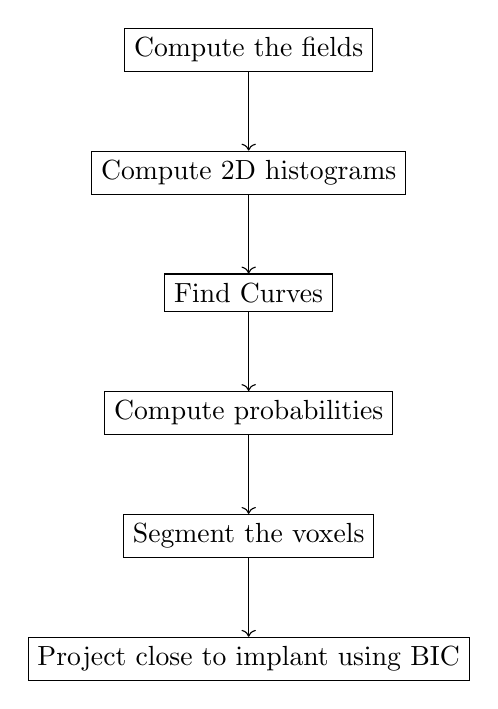
\begin{tikzpicture}
        \node[draw] (field) at (0,0) {Compute the fields};
        \node[draw, below = of field] (hists) {Compute 2D histograms};
        \node[draw, below = of hists] (curvs) {Find Curves};
        \node[draw, below = of curvs] (probs) {Compute probabilities};
        \node[draw, below = of probs] (segm) {Segment the voxels};
        \node[draw, below = of segm] (bic) {Project close to implant using BIC};

        \path[draw, ->] (field) -- (hists);
        \path[draw, ->] (hists) -- (curvs);
        \path[draw, ->] (curvs) -- (probs);
        \path[draw, ->] (probs) -- (segm);
        \path[draw, ->] (segm) -- (bic);
    \end{tikzpicture}
    \caption{Flowchart depicting the steps of the method. 
    \carl{Skal nok labeles, så man nemt kan se hvilken section der beskriver det. Plus, teksten i kasserne nok også kan være mere flavorful!}
    \carl{Kan måske arrangeres ligesom Davids ting oversigt? Giver måske kun mening hvis der var mere end bare segmentation -> bic}}
    \label{fig:flowchart}
\end{figure}

\subsubsection{Segmentation}

\begin{description}
    \item[Field-computations]

    EDT

    Diffusion

    EDT + Diffusion

    (remember to show images)

    \item[2D histograms]

    \item[Curves]

    \item[Probabilities]
\end{description}

\subsubsection{BIC computations}

\subsection{Results of the field segmentation}


\section{Verification and analysis}
\label{sec:verification}

In this section, we present the verification of the segmentation method
described in \Cref{sec:method}. First we qualitatively verify that our method
is sound by comparing the segmentation results to the original tomography and
creating an artificial ground truth. Then we quantitatively verify our method
by generating synthetic data, evaluating it on the created ground truth, and
comparing the results to other existing methods. Finally, we analyze the
segmented data to study the blood vessel network in the bone region and produce
statistics on the tissue-to-implant contact.

\subsection{Qualitative verification}

Since the SRµCT tomograms are clear enough that humans can distinguish between
blood vessels and bone, as our mammalian visual cortex automatically corrects
for the distortion effects, we can verify the success of the automatic
classification. We can compare the automatic classification with the manual
classification of the histological microscopy. A larger quantitative study is
planned that analyses the full data set against recently conducted histological
microscopy taken from the same biopsies. As such, we can only present a
qualitative verification of the method in this paper.

Figures \Cref{fig:histology-comparison1} and \Cref{fig:histology-comparison2}
show the same 2D slices as were shown in Figures \Cref{fig:3viewsample} and
\Cref{fig:slices}, allows us to visually inspect them side by side. The voxels
are colored according to the segmentation confidence, with the degree of red
being proportional to the modeled probability $\Pof{0}{v,\fval}$ and the degree
of yellow being proportional to $\Pof{1}{v,\fval}$. Grey voxels indicate low
model probabilities of both: either due to the voxel belonging to another
material or simply low computed confidence of the model. By comparing Figures
\Cref{fig:histology-comparison1} and \Cref{fig:histology-comparison2}, we see
that the computed classification matches the human classification everywhere
where it is possible to visually distinguish the voxels.

\begin{figure*}
    \centering
    \begin{tabular}{cc}
        \includegraphics[width=.45\linewidth]{generated/770c_pag_segmented_yx_raw.pdf} &
        \includegraphics[width=.45\linewidth]{generated/770c_pag_global_yx_otsu.pdf}
        \\
        \includegraphics[width=.45\linewidth]{generated/770c_pag_segmented_yx_colored.pdf} &
        \includegraphics[width=.45\linewidth]{generated/770c_pag_global_yx.pdf} \\
    \end{tabular}
    \caption{
        YX slices of the original tomography (top left), our classification
        (bottom left), and global threshold classification (bottom right). For
        our classification, the voxels are colored according to the modeled
        probability functions $P(m\vert v,\fval)$ between 0 and 1: completely
        red voxels have $P(m=0\vert v,\fval) = 1$, completely yellow voxels
        have $P(m=1\vert v,\fval)\ = 1$, and uncertain voxels become
        progressively gray.
    }
    \label{fig:histology-comparison1}
\end{figure*}

\begin{figure*}
    \centering
    \begin{tabular}{cc}
        \includegraphics[width=.45\linewidth]{generated/770c_pag_segmented_zy_raw.pdf} &
        \includegraphics[width=.45\linewidth]{generated/770c_pag_global_zy_otsu.pdf}
        \\
        \includegraphics[width=.45\linewidth]{generated/770c_pag_segmented_zy_colored.pdf} &
        \includegraphics[width=.45\linewidth]{generated/770c_pag_global_zy.pdf} \\
    \end{tabular}
    \caption{
	    YZ slices of the original tomography (top left), Otsu segmentation
	    (top right), our classification (bottom left), and global threshold
	    classification (bottom right).  Yellow depicts bone and red depicts
	    soft tissue. Note that our segmentation correctly classifies the
	    materials close to the implant, even in the grooves of the screw
	    threads, whereas the global threshold classification fails.
    }
    \label{fig:histology-comparison2}
\end{figure*}

We see that the segmentation is overall successful, classifying the internal
darker regions as soft tissue and the lighter regions as bone. This is further
confirmed in \Cref{sec:blood-network}. However, extremely close to the implant
(a few voxels), we cannot verify the segmentation, as the voxel values are so
blended together with the implant voxel values that they become
indistinguishable. A further strengthening of the analysis is needed to reach
this layer. It is possible that the information is irretrievably lost, or
perhaps it can be retrieved through a deconvolution - or simply a more precise
version of the present analysis. It also fails within some of the soft tissue
blobs, which is due to air bubbles in the resin, which have a very low density
and thus a very low absorption.

\subsection{Quantitative evaluation}

% Why it is a problem
Reliably evaluating segmentation methods on medical data such as that
presented in this paper is a challenging task. A satisfactory annotated ground
truth does not exist, which makes quantitatively evaluating one method against
another very hard. Furthermore, due to the very large number of voxels, using
manual or semi-automatic methods quickly becomes impractical. One such example
are neural networks, which need to be trained on multiple instances of similar
data accompanied by an annotated ground truth. This is a very time consuming
and expensive procedure, and does not easily translate to other data, which are
only slightly dissimilar.

In order to ensure a reliable and consistent verification of our method, we
must tackle a common problem in medical physics. Namely that problems are often
solved using approaches which can be hard to reproduce and therefore
verify~\cite{replication-crisis}. We try to overcome this difficulty by
creating synthetic reproducible data, accompanied by a consistent reference
level ground truth. The generated data resembles our original data and shares
many physical qualities, but instead of being acquired at ESRF, it is simulated
using the software Novi-sim~\cite{novisim} on an affordable workstation using a
consumer-grade GPU (Nvidia RTX 3080). This allows other researchers to not only
reproduce but also modify our tomographic models and perform new experiments.
This attempts to both extend the robustness of our proposed method, and make it
less specific and dependent on our original data. In future experiments this
also allows to extract 2D-slices of synthetic data and compare with manually
inspected and annotated histologies.

Original data and synthetic data, with STL files and ground truth are available
at github link.
% TODO: add link

\subsubsection{Ground truth and synthetic data}

% How we use Novi-sim
The presented segmentation pipeline results in a set of masks, one for each
material.  Each mask is overlayed unto a single volume representing our
artificial ground truth. By construction it will have a perfect overlap,
correctly identifying each material using our method.  Furthermore the masks
for each material are converted into meshes and used to generate STL files.
The generated STL files are transformed to synthetic tomograms using Novisim.
While the software is set up to simulate the original experiment at ESRF, it
will naturally not be a perfect match. The generated ground truth is now
perfectly accurate with the input, but deviates slightly but predictably from
the generated tomogram due to experimental physical effects and artifacts. This
allows us to use reproducible synthetic data to consistently compare our
segmentation method with other, and also detect in which regions they differ
the most. Since we expect regions very close and very far away from the implant
to be difficult, any intermediate regions should be fairly consistent across
methods. Finally we can inspect the differing regions visually to evaluate on
the overall performance.

\subsubsection{Comparison to other methods}

Having a reproducible tomogram with corresponding ground truth, allows us to
make a comparison to other methods. The simplest approach is having a global
threshold. This is used to illustrate why we cannot afford to rely on too
simple methods.  Next we show how a more flexible multi-level automatic Otsu
segmentation performs and its drawbacks. Finally we look at fully automatic
ML-based methods and illustrate the assumptions that underlie their peformance
and how they are not always sufficient or practical for data similar to ours.

\subsection{Dataset analysis}

Having verified the method qualitatively and quantitatively, we can have a more
detailed look into the segmented data. We are interested in the blood vessel
network in the bone region and the tissue-to-implant contact. We will start by
analyzing the blood vessel network and then the tissue-to-implant contact.

\subsubsection{Blood vessel network}
\label{sec:blood-network}

With a good separation of soft tissue and bone, we map out the blood vessel
network using connected components analysis, which is visualized in the 3D
renders in~\Cref{fig:blood-network}. Here we see that we have successfully
segmented the blood vessels out of the bone region. It is especially prominent
when looking at the capillary network, as we can see these in fine detail.
Noteworthy, the newly formed bone region (\Cref{fig:blood-new-slice}) contains
larger concentrations of small blood vessels, compared to the old bone
(\Cref{fig:blood-old-slice}). If we zoom in on a small cube region
(\Cref{fig:blood-old-cube} and \Cref{fig:blood-new-cube}), we see it even more
defined, clearly seeing how the larger vessels connect through the smaller
ones.

\begin{figure}
    \centering
    \begin{subfigure}[b]{\linewidth}
    \centering
        \includegraphics[width=.7\linewidth]{generated/figure10_old_bone.png}
        % TODO opdater hvis en anden slice størrelse bliver brugt. voxel size = 3.75
        \caption{A 375 µm $\times$ 4230 µm $\times$ 6480 µm slice of the blood network in the old bone region.}
        \label{fig:blood-old-slice}
    \end{subfigure}
    \begin{subfigure}[b]{\linewidth}
    \centering
        \includegraphics[width=.7\linewidth]{generated/figure10_new_bone.png}
        \caption{A 375 µm $\times$ 4230 µm $\times$ 6480 µm slice of the blood network in the new bone region.}
        \label{fig:blood-new-slice}
    \end{subfigure}
    \begin{subfigure}[b]{.48\linewidth}
    \centering
        \includegraphics[width=.9\linewidth,height=\linewidth]{generated/figure10_old_cube.png}
        \caption{A $1mm \times 1 mm \times 1 mm$ cube of the blood network in the old bone region.}
        \label{fig:blood-old-cube}
    \end{subfigure}
    \hfill
    \begin{subfigure}[b]{.48\linewidth}
    \centering
        \includegraphics[width=.9\linewidth,height=\linewidth]{generated/figure10_new_cube.png}
        \caption{A $1mm \times 1 mm \times 1 mm$ cube of the blood network in the new bone region.}
        \label{fig:blood-new-cube}
    \end{subfigure}
    \caption{
        3D renders of the blood network. We see a difference between the
        capillary network in the old bone region
        (\ref{fig:blood-old-slice},\ref{fig:blood-old-cube}) compared to the
        newly grown bone region
        (\ref{fig:blood-new-slice},\ref{fig:blood-new-cube}), where the new
        bone region contains a higher concentration of small blood vessels,
        compared to the old bone region containing fewer larger blood vessels.
    }
    \label{fig:blood-network}
\end{figure}

\subsubsection{Implant contact}
\label{sec:contact}

Tissue in contact with the implant can be studied using the EDT from the
implant, restricted to the bone region. We can simply mask the voxels that are
within a thin shell of distances, $d_{min} < d(x,y,z) \le d_{max}$, for
example, $d_{min} = 1 \text{µm}$ to $d_{max} = 5 \text{µm}$. We then sum over
the masked voxels of each tissue type to obtain and divide by the total to
obtain the tissue-to-implant contact per area or study the distribution across
the surface area qualitatively. In particular, we are interested in the
difference between the old and new bone regions. We define the metric as
follows:

\begin{equation}
    BIC = \frac{\sum_{i : \text{field}(i) < 5} \text{bone}(i)}{\sum_{i : \text{field}(i) < 5} \text{voxels}(i)}
\end{equation}

We find the old and new bone regions at different $z$ levels, based on the
threading of the implant, with new bone being near the small threads and old
bone being near the large threads. The results can be seen in \Cref{tab:bic}.
We see that the BIC is higher in the old bone region than in the new bone
region, which is expected as the bone grows around the implant over time. This
is further confirmed by the blood vessel network analysis, as the new bone
region contains a higher concentration of small blood vessels, indicating that
the bone is still growing. This shows that the method is successful in
segmenting the bone and soft tissue regions and that the segmentation can be
used to study BIC.

\begin{table}
    \caption{The mean and standard deviation of bone-to-implant contact in the old and new bone regions for each of our samples.}
    \label{tab:bic}
    \centering
    \begin{tabular}{lcc}
        \toprule
        Sample & Old bone & New bone \\
        \midrule
        770\_pag & $0.5020 \pm 0.1222$ & - \\
        770c\_pag & $0.6519 \pm 0.1055$ & $0.5638 \pm 0.0907$ \\
        771c\_pag & $0.4517 \pm 0.1708$ & $0.5016 \pm 0.1078$ \\
        772\_pag & $0.7012 \pm 0.1065$ & $0.5222 \pm 0.0869$ \\
        775c\_pag & $0.2802 \pm 0.0928$ & $0.2652 \pm 0.1054$ \\
        810c\_pag & $0.6819 \pm 0.0866$ & $0.5155 \pm 0.0897$ \\
        811\_pag & $0.5832 \pm 0.1015$ & $0.3715 \pm 0.0935$ \\
        \bottomrule
    \end{tabular}
\end{table}


\section{Conclusion and future work}
\label{sec:conclusion}

While SR$\mu$CT yields 3D reconstructions of extremely high fidelity compared to lab-grade X-ray setups,
several distortion effects remain that obstruct accurate tissue classification in important regions, in particular
near and at interfaces of high-contrast transitions such as where biological tissue meets metallic implants.
However, these effects are well behaved, in the sense that they vary smoothly over space, making it possible
to discover approximate mathematical models of the effects, and counter their resulting distortion.

We were able to build probabilistic models for the distortive effects
of soft tissue and bone voxel values as functions of distance to the
implant, and as functions of an approximate diffusion field. This made
it possible to see all the way up to the implant surface, and
automatically segment into tissue types throughout the sample and all
the way up to the implant surface, with high accuracy both at long and
short distances.

In this pilot work, we have only made a qualitative study. In upcoming
work, we plan a larger quantitative study that compares with histology
microscopy results, obtained from the same biopsies.  In addition, we
are extending the method with Bayesian combination of multiple
``angles'': different sources of distortion effects (e.g.~multiple
physical effects) can be better captured by different fields,
e.g.~beam hardening may be best captured by the distance transform to
the sample surface, while the diffusion field captures distortion near
metallic implants. Thus different fields separate tissue material
distributions in different regions, and in combination are expected to
yield a stronger analysis. It is hoped that this will make it possible
to separate multiple highly overlapping frequency distributions.


\section{Acknowledgements}

This project has received funding from the European Union’s Horizon 2020 research and innovation programme under grant agreement No. 779322 (``MAXIBONE'').
JA was partially supported by the VILLUM Foundation through VILLUM Experiment Project: 41017.
CJ was funded by the Innovation Fund Denmark (IFD) under File No. 8057-00012B, the IFD Grand Solutions project ``Adaptive X-ray InSpection''.

\section{Conflict of Interest}
On behalf of all authors, the corresponding author states that there is no conflict of interest. 


%%% Local Variables:
%%% mode: latex
%%% TeX-master: "main"
%%% End:


% ---------------------------------------------------------------------------- %

\bibliography{sn-bibliography}% common bib file

\end{document}
